\documentclass[format=acmlarge, nonacm=true]{acmart}

\usepackage{siunitx, booktabs}

\usepackage{amsmath}

\usepackage{hyperref}

\usepackage{graphicx}
\usepackage{caption}
\usepackage{subcaption}

%opening
\title{Search-Based Robust XPath Generation}
\author{Chanyoung Ryu}
\affiliation{KAIST Department of Computer Science}

\author{Chanmin Park}
\email{cmpark0917@kaist.ac.kr}
\affiliation{KAIST Department of Computer Science}

\author{JeongHo Ha}
\email{hajh@kaist.ac.kr}
\affiliation{KAIST Department of Computer Science}

\author{Sangwoo Hahn}
\email{thahn106@kaist.ac.kr}
\affiliation{KAIST Department of Computer Science}

\date{\today}

\authorsaddresses{}

\begin{document}

\maketitle
\section{Introduction}
In web design, developers need the ability to make quick updates to websites while retaining prior functionality. A key part of the development process is automated regression testing, in which a website’s functionality is verified to work despite changes. Elements of a website are found using XML Paths (XPaths), which locates elements by representing them with relative or absolute paths, similar to those used in file systems. XPaths are reliable in locating elements in static websites, but as a website's structure changes, they may not be able to locate the same elements. Therefore, a key problem in automated web regression testing is to find XPaths that can survive version changes, also known as robust XPaths.\\
A greedy algorithm approach is able to generate optimal robust XPaths by searching through the entire set of possible XPaths. However, this set increases exponentially with the number of attributes in an element and the number of elements in a webpage, deeming this approach impractical. Other search-based approaches have been proposed to generate less-than-optimal XPaths but no empirical tests have verified the validity of these claims.\\
In this paper, we propose a genetic algorithm to generate robust XPaths. Among other search-based methods, a genetic algorithm is a good fit as mutation and crossover operators are clearly defined and enable the exploration of the entire search space. The genetic algorithm was able to find a robust XPath for the majority of the target elements, including many that had their structures changed. The genetic algorithm was favorable in performance compared to the XPaths automatically generated by Google Chrome, and was able to perform reasonably well across different types of DOM structures. \\
An overview of the paper goes as following: in Section 2, background information is provided and the terminology used in the paper is defined; in Section 3, previous works and their limitations are outlined; in Section 4, components of the genetic algorithm, such as selection methods and exploration operators, are described in detail; in Section 5, the dataset used for evaluation is described; in Section 6, the performance of our algorithm is evaluated against a commercial XPath generator; and in Section 7, conclusions and potential future works are discussed.\\

\section{Background}
Web pages are represented as document object model (DOM) trees, where each element is a node in the tree. Developers must find a way to represent and locate these elements to perform automatic testing. Among various methods such as regular expressions and CSS selectors, XPaths exploit the tree structure to represent elements in an intuitive yet precise manner. They allow for a relative search anywhere in the document for elements that result in a match. For example, “//html/div[@class=‘X’][1]/p[@id=‘Y’]” represents finds all ‘p’ tag elements with an ID value of ‘Y’, under the first ‘div’ tag with class name ‘X’ under its parent, under an ‘html’ tag.  For the purposes of this paper, an XPath consists only of tags and attributes, where attributes include class name, ID value, and position under its parent.\\
When an XPath uniquely identifies an element in the web page, it is a locator for that element. For static websites, any XPath that is a locator can be used for testing. However, modern websites undergo frequent updates that may change the DOM tree. This implies that an XPath must also be able to locate the same element in future versions of a website for effective regression testing. Otherwise, a new XPath must be generated and validated, adding an entire layer of uncertainty. Therefore, generating robust XPaths, those that are able to locate the same element despite changes to the website structure, is an important task in web development.\\
To evaluate the robustness of an XPath, a metric called the fragility coefficient is defined to measure the fragility (inversely proportional to robustness) of an XPath. Intuitively, it would be the case that certain parts of an XPath make it more fragile; for example, adding a position attribute to an XPath will make it more fragile, since inserting or removing an element above the target element likely prevents the XPath from locating the same element. Thus, a weight proportional to fragility is associated with each part of an XPath, and these weights are summed to generate a fragility coefficient for an XPath. These weights are not defined, so a significant part of the evaluation was dedicated to determine them. Further details are provided in Section VI.\\

\section{Related Works}
There have been several studies in attempt to generating robust web element locators in the effort of reducing web test suite maintenance work due to structural changes. Among many different kinds of locators for web page elements, many of the studies have focused on XPath locators for following reasons.
\begin{enumerate}
	\item XPath locators are highly expressive, since most of the other localization methods provided by DOM-based tools can be simulated using XPath expressions.
	\item XPath locators are sometimes the only option as some localization methods are applicable only to specific cases.
	\item XPath locators are generally considered fragile, but this strongly depends on how they are created.	
\end{enumerate}
A recent work presented ROBULA (ROBUst Locator Algorithm), a tool that implements a heuristic to generate robust Xpath locators [1]. While preliminary results with ROBULA are quite promising, the heuristic approach implemented in ROBULA suffers two main problems: 1) there may exist cases in which it does not return any locator in reasonable amount of time, because of the exponential complexity of the heuristic it implements; 2) it may return a suboptimal locator even when it has enough time to compute it, because it is not guaranteed to return optimal locator in case of convergence. As a supplementary to the deterministic heuristic, the authors of ROBULA proposed a meta-heuristic algorithm that formulates the robust locator generation problem as a graph search problem, so as to make it treatable by means of genetic algorithm [2]. This formulation served as the motivation for this empirical study.

\section{Methodology}
This section provides a detailed look at the formulation of the genetic algorithm.
Chromosome: a chromosome is an XPath.\\
Population: a population is a set of chromosomes; that is, a set of XPaths. Furthermore, two sub-populations are distinguished since separate fitness functions must be used for each:
\begin{itemize}
\item pop’: the set of XPaths that are not locators of the target element; that is, it locates two or more elements in the DOM tree.
\item pop’’: the set of XPaths that are locators of the target element.
\end{itemize}
The initial population is generated with following three types of XPaths:
\begin{enumerate}
	\item “//*” – the most generic XPath
	\item The full absolute XPath – the XPath containing every attribute from every level to the target element
	\item XPaths generated by removing highest layer of the full absolute XPath one at a time
\end{enumerate}
Fitness function: the fitness is defined separately for the two sub-populations:
\begin{itemize}
	\item pop’: number of elements located by the XPath.
	\item pop’’: the fragility coefficient described in Section VI.
\end{itemize}

It is important to note that when comparing an element from pop’ and an element from pop’’, the latter has a lower fitness score; that is, XPaths that are locators are always preferred over non-locators.\\
Parent selection: tournament selection with a tournament size of 3 is used to select parents. Tournament selection is preferred over fitness proportional selection or ranking selection due to its balance between exploration and exploitation when applying evolutionary pressure.\\
Generational selection: modified generational replacement is used to select children, the modification being that the initial population is always retained in every generation. Since the initial population exhibits great diversity, from the most generic XPath to the most specific locator, it is maintained in every generation to guarantee diversity. Elitism is an alternative to generation replacement. However, when keeping the select best from the parents, XPaths in pop’’ would always be ranked higher than pop’. Thus, those in pop’ would not be able to survive many generations, significantly reducing the diversity of the population.\\
Mutation: a total six mutations, three pairs of two complementary mutations, are defined. The set of mutations are described in Figure 1.a.\\

Crossover: only single-point crossover is defined. Given two parent chromosomes, this crossover method randomly chooses a level from the bottom, splits the chromosomes, and recombines them. An example of a crossover operation is shown in Figure 1.b.\\

\begin{figure}
	\centering
	\caption{Evolutionary operators}
	\begin{subfigure}{.5\textwidth}
		\label{tab:conf}
		\resizebox{\columnwidth}{!}{%
			\begin{tabular}{ll}
				\toprule
				\emph{trans\_add\_name} & replaces the * in the highest level to a specific tag \\
				\emph{trans\_remove\_name} & replaces a specific tag in the highest level to a *\\
				\midrule
				\emph{trans\_add\_predicate} & adds a predicate to the highest level \\
				\emph{trans\_remove\_predicate} & removes a predicate at the highest level \\
				\midrule
				\emph{trans\_add\_level} & adds a new * level\\
				\emph{trans\_remove\_level} & removes the highest level\\
				\bottomrule
			\end{tabular}
		}
		\caption{Mutation Operations}
	\end{subfigure}%
	\begin{subfigure}{.5\textwidth}
		\centering
		\label{fig:test}
		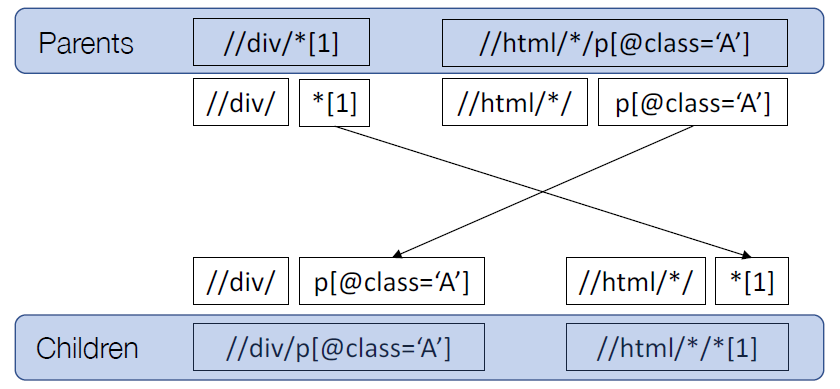
\includegraphics[width=.8\linewidth]{images/crossover.png}
		\caption{An example of a crossover operator}
	\end{subfigure}
\end{figure}

Parameters: the parameters are set as shown in Table 1.\\

\begin{table}
	\label{tab:para}
	\caption{GA hyperparameters}
	\begin{tabular}{ll}
		\toprule
		Max Population & 50 \\
		Max Evaluations & 10000\\
		Mutation Rate & 0.3\\
		Crossover Rate & 0.8\\
		\midrule
		Selection Method& Tournament Selection\\
		Generational replacement & Maintain original population\\
		\bottomrule
	\end{tabular}
\end{table}






\section{Dataset}
\subsection{Test Subjects}
The test subjects of our XPath locator are html files of websites since the locator is DOM-based. We have devised some conditions that must be satisfied to work as a test dataset of this XPath locator. The conditions are as follows:
\begin{enumerate}
	\item It should have both the old and new version of the website, which has undergone a structural change during the time gap.
	\item It should have a same element, in both the old and new version of the website. 
\end{enumerate}
An element could range from text of an article/post, to image or video files. However, in our test dataset, selected target elements used are texts. This is because text elements in the DOM are generally more concise and shorter than image elements.



\subsection{Data Collection}	
The test datasets are collected from <Internet Archive Wayback Machine> . We collected a total of 18 test sets of various types. The types include news articles, social network services, enterprise’s official website…etc. We divided the test sets into two types, which are as follows:
\begin{itemize}
	\item \emph{Type 1:} Google chrome XPath from old version can locate designated element in the new version.
	\item \emph{Type 2:} Google chrome XPath from old version cannot locate designated element in the new version.
\end{itemize}

\begin{figure}
	\centering
	\label{fig:test}
	\caption{A webpage with both type 1 and type 2 element}
	\begin{subfigure}{.5\textwidth}
		\centering
		
\includegraphics[width=0.8\linewidth]{images/FB1.png}
		\caption{An element of Type 1}
		\label{fig:sub1}
	\end{subfigure}%
	\begin{subfigure}{.5\textwidth}
		\centering
		
\includegraphics[width=.8\linewidth]{images/FB2.png}
		\caption{An element of Type 2}
		\label{fig:sub2}
	\end{subfigure}
\end{figure}

This we because we wanted to check if our locator is at least as good as Google chrome locator by passing all test cases from type 1, and hopefully show better performance by passing some of the test cases from type 2. Of the 18 test datasets, 5 of them are type 1 and the other 13 are type 2. The 2016 Facebook main page is a special test case because it contains both type 1 and type 2 elements. 


\section{Evaluation}
\subsection{Parameters}
As the reference paper only supplied an approach for the genetic algorithm rather than the specifications, it was necessary to choose the parameters for the genetic algorithm and the fitness function. The fitness function can be represented as a vector in $\mathbb{R}_+^5$ as each of the mutations results in a *, label, index id, or class, with each of them having a specific cost assigned to it. Random weight sets were created by sampling from $[0,10]$. In most cases, the fitness values tended to converge around 1,500 to 3,000 evaluations, so 3,000 was used as the baseline for picking the best fitness function. However, since a higher percentage of GAs were fully convergent by 10,000, 10,000 was set as the default parameter for the main execution. Other GA hyperparameters were set based on the rate of convergence.\\

500 different 5-tuples of $[0,10]$ were tested as fitness function values. No single GA covered more than 9 cases, but of the top 10 GAs in terms of coverage, there was subset of three GAs that covered all the cases covered by at least 1 GA, which are the cases are known to have a robust XPath. Table 2 shows the three fitness function that combined, cover all known cases.\\

\begin{table}
	\label{tab:cover}
	\caption{GA Fitness Functions}
	\begin{tabular}{l|lllll}
		\toprule
			&	*& tag& position& class& id\\
		\midrule
		GA 1& 5.2& 1.8& 4.8& 8.8& 8.0\\
		GA 2& 2.1& 9.5& 3.5& 6.1& 7.8\\
		GA 3& 7.5& 9.1& 4.4& 9.6& -2.1\\
		\bottomrule
	\end{tabular}
\end{table}


\subsection{Coverage}
\begin{table}
	\label{tab:cover}
	\caption{Test Data Coverage}
	\begin{tabular}{lll|lll|l}
		\toprule
		Source&	Type&	Date Retrieved&	GA 1&	GA 2&	GA 3&	Covered\\
		\midrule
		BBC&2&2015&TRUE&FALSE&FALSE&TRUE\\
		CNN&2&2012&FALSE&FALSE&FALSE&FALSE\\
		Donga Science&2&2016&FALSE&TRUE&FALSE&TRUE\\
		Facebook&2&2010&FALSE&FALSE&FALSE&FALSE\\
		Nature&2&2013&TRUE&TRUE&TRUE&TRUE\\
		NY Times&2&2014&FALSE&FALSE&FALSE&FALSE\\
		Reuters&2&2016&FALSE&TRUE&FALSE&TRUE\\
		Foxnews&2&2015&TRUE&FALSE&FALSE&TRUE\\
		Facebook&1&2016&TRUE&TRUE&TRUE&TRUE\\
		Apple&1&2016&FALSE&FALSE&FALSE&FALSE\\
		IEEE&1&2015&TRUE&TRUE&TRUE&TRUE\\
		King's College London&1&2016&TRUE&TRUE&TRUE&TRUE\\
		Wall Street Journal&1&2016&TRUE&FALSE&FALSE&TRUE\\
		NY Times&2&2015&TRUE&FALSE&TRUE&TRUE\\
		Porsche&2&2014&TRUE&TRUE&TRUE&TRUE\\
		Rolex&2&2015&FALSE&TRUE&FALSE&TRUE\\
		Github&2&2017&FALSE&FALSE&TRUE&TRUE\\
		Facebook&2&2016&FALSE&FALSE&TRUE&TRUE\\
		\bottomrule
	\end{tabular}
\end{table}

The genetic algorithm was generally superior to the baseline Google Chrome algorithm, covering 14 out of 18 as opposed to 5. While no single GA covered more than 9, the combination of three GAs were sufficient in covering most of the cases. Since no locator returned by the algorithm returned a different element in the new version, a naive approach to using these locators is taking all three and trying them one by one. However, this may have simply been a coincidence and there is no guarantee that if a locator returned by the GA finds a unique element it is the element we are looking for. Fortunately, in actual use, the test suite used for automated regression testing would be able to detect that.\\
The different GA fitness functions had different evolutionary pressures, leading to different optimal xpaths. For example, GA 1 has very low cost in adding tags, so deeper structures with many tags would have an evolutionary advantage. Since GA 3 has a negative cost for ids, the algorithm would be encouraged to label ids when it can. However, since the cost of ``*  + id'' or ``tag + id'' is still positive, it would actively add levels just to add more ids. 

\subsubsection{Failed Cases}
Only three cases were missed by all three GAs and the Google algorithm. Of those three, two were from 2010 and 2012, and the website designed changed too much to locate the same element. There might be no robust XPath that could be derived from the old html file.\\

In the last one that was missed by the GAs, the key tags surrounding the date element in question were changed. All the genetic algorithms found a "robust" solution that used a nearby tag, and therefore were not able to locate the target element in the new version.\\

\subsubsection{Performance}
Given a DOM and a target element, the algorithm typically took 8 to 12 seconds to generate the robust locator. Since finding the desired target element in a html file and porting the path typically takes about 30 seconds, the amount of time saved by automating this can be estimated to be $(30\text{ secs})\times \%coverage\times (\#\text{ of tests})$. If we assume a web testing suite needs just 50 locators and since our coverage rate is 87\%, one can save roughly 20 minutes every time tests need to be performed. A more accurate analysis of time savings could be calculated if the breakage rate of elements of interest is performed, but currently there is no well-defined parameters for elements of interest, and the domains are too wide.


\section{Future Work}
We have formulated the problem of generating robust XPath locators as a graph search problem, for which we have provided and tested a meta-heuristic solution based on a genetic algorithm. While the empirical evaluation showed promising results, the scope of the analysis was very limited as only 18 target elements in total were tested. We could add more test data to have a more thorough analysis, and more versions of a given website could be tested. In addition, adding more complexity to the predicate candidates by exploiting on text or subset of classes might be beneficial in generating more robust XPaths.\\ 

The tested fitness function was simply a weighted sum of all the operations applied with no regards to the levels involved. A given type of operation had the same cost regardless of the level it was involved in. One of the ways this project can be extended is to have a dynamic weighting across the various DOM levels so that more nuanced structures can be optimized for by the genetic algorithm.\\

Another possible extension is by using the nested nature of websites to learn the structure. The main problem with a partially matching robust XPath is that if additional levels are added or removed between the top and bottom level of the XPath, it is likely to break immediately. One of the most common changes in website design are addition and removal of formatting levels, so it would be useful to have a robust locator that takes those changes into account. By finding a top level element that we know our target element to belong to and searching within that element with a second locator might allow for the exploitation of the common nesting models of website design.\\

Moreover, applying hyper-heuristic to attain fitness function weights might be able to prevent fitness function from prioritizing DOM structures specific to test cases. Analysis on more than one past versions of websites might be meaningful in scoring fitness for XPath robustness throughout hyper-heuristic iterations. \\
Our study on robust XPath generation has suggested that websites that preserved modular structure despite major changes in to DOM structure had higher tendency to have a robust XPath. Also, we witnessed that some ill-practiced inconsistent CSS class names (e.g. class=“akfhg3kn”) often fail the generated XPaths. It would be a good practice in web design engineering to use meaningful and consistent naming schema, and maintain modular structures. \\




\section*{References}
\begin{enumerate}
	\item M. Leotta, A. Stocco, F. Ricca, and P. Tonella. Reducing web test cases aging by means of robust XPath locators. In Proceedings of 25th International Symposium on Software Reliability Engineering Workshops, ISSREW 2014, pages 449–454. IEEE, 2014.
	\item M. Leotta, A. Stocco, F. Ricca, and P. Tonella. Meta-heuristic generation of robust XPath locators for Web testing. In SBST, pages 36–39, May 2015.
\end{enumerate}

\newpage
\section*{Github}
\url{https://github.com/chandescartes/cs454/}
\begin{itemize}
	\item Chanmin Park: porkyeye
	\item JeongHo Ha: Ha-JH
	\item Chanyoung Ryu: chandescartes
	\item Sangwoo Hahn: thahn106
\end{itemize}
\end{document}
